\chapter{Introduction} %5523
\label{ch:intro}
The discipline of archaeology analyses the traces left by people in the past, traces left in both space and time. While the study of spatial data in archaeology is a long one with a considerable literature, the study of temporal data might be considered the poor relation. In fact \citet{Lucas:2005fk} states that a ``proper examination of the concept of time in relation to archaeological theory and method did not really begin until the late 1970s and 1980s'' \citep[28]{Lucas:2005fk}. This situation is now changing e.g. \citet{Bailey:2007fk, CAJ:676016, Bolender:2010po, eps376489} etc. and there is now a wide front on which to engage with time. 

\citet{Lucas:2005fk} divides divides this front along the lines of \citet{Leone:1978fk} and \citet{Bailey:1981uq, Bailey:1983kx}, into archaeologists' perception of time, and past societies' perception of time. With regard to the former a significant amount of work has been undertaken on the use of mathematical techniques to refine dates, in particular radiocarbon dates. A key element of this is known as bayesian modelling, due to its use of bayesian statistical techniques, stemming from \citet{Bayes:1763fk}. The method as used by archaeologists can be traced back to \citet{Buck:1991fk} and see \citet{Buck:1996oq,Buck:2004uq} for more detailed descriptions of the technique. With regard to past societies' perception of time, there has also been the development of a considerable body of literature, for example \citet{Bradley:2002fk}.

This thesis evaluates the state of the art of spatio-temporal method and theory. It will examine how archaeologists deal with time, in particular, how to handle and analyse spatio-temporal data and how it is represented and reproduced. Fundamentally, it will question whether modern temporal techniques lack a consideration of the spatial context, what the negative consequences of this might be, and how space and time may be re-combined.

In order to contextualise this investigation with a site that has been intensively studied, consider Hambledon Hill. Hambledon Hill is a site that will be returned to throughout this study, making particular use of the detailed volume of \citet{Mercer:2008fk}. Very briefly, Hambledon Hill is a site of intense Neolithic activity, including causewayed enclosures, long barrows and defensive earthworks \citep[xiii]{Mercer:2008fk} in South West England. Between 1974 and 1986 Roger Mercer directed a programme of excavation the result of which is the published volume, \citet{Mercer:2008fk}.

The long program of research at the site has created a vast amount of data, but with regard to the temporal data, this falls into several general categories. The field survey \citep[15]{Mercer:2008fk} reports time as the relationship between features, (i.e. earlier/later) while the excavation \citep[41]{Mercer:2008fk} deals with time as probabilistic dates (from radiocarbon determinations) and in relative terms from the stratigraphy. While this last form of temporal data is similar in some ways to the relationships between features in the field survey, it is operating on a different scale. The stratigraphic relationships are also routinely grouped, for example finds and contexts grouped into phases, and in addition there is the difference that phases are referred to by numbers, so there is an inherent ordering. 

Broadly, then, this is in line with the ontology of relative and absolute time, or abstract and substantive time \citep{Lucas:2005fk}. However, it is worth considering if this has to be the case. As Lucas points out, this distinction is perhaps misguided \citep[93]{Lucas:2005fk} as our abstract or absolute time is often loaded with meaning. We must remain aware that our abstract dates also carry subjective connotations for us. Pragmatically however, the types of data that we are dealing with are very different. What one might term absolute dates are of a more numerical form, where as relative dates are a relationship. The absolute, relative division of time is valuable to note the distinction in data, but clearly less so in terms of chronotypes \citep{Lucas:2005fk}.

These two different types of temporal data are used in different, often complementary ways. At Hambledon the relative information from the field survey was used to piece together an idea of the ordering of the use and re-use of the site, for example, this temporal information is used to conclude that a field system pre-dates a Neolithic earthwork, as the field alignment does not follow the earthwork axis \citep[29]{Mercer:2008fk}. However, relative information from the section of an excavation is used to counter this argument, as it demonstrated levelling of banks, and plough soil over the ditches \citep[29]{Mercer:2008fk}. The relative temporal information from the excavation is used to order phases, often given a period, such as Neolithic or fourth millennium BC e.g. \citet[44]{Mercer:2008fk}. They are also associated with artefacts, which can sometimes be dated using an absolute method.

At Hambledon many artefacts were radiocarbon dated, these dates are then used to provide an additional temporal dimension to the phases, based on the abstract radiocarbon scale, or calibrated to calendar years (another abstract representation of time). Such dates are taken from samples throughout the phases and contexts, being used to tie these entities into the abstract chronology of our temporal system. As the authors note, the dates provided by this technique are of the sample (rather than the whole phase) and ``it is the dates of the archaeological events represented by those samples that are significant'' \citep[378]{Mercer:2008fk}. However this presents a problem, the event itself may have been a short lived event, it may have only taken minutes to occur, but the imprecision of radiocarbon dating is such that there may only be an accuracy of a hundred years or so. In addition, there will also be some uncertainty attached to the date, often reported as a confidence percentage, which is due ultimately to the measurement error. These two factors combined mean that the result of such analysis is temporal data of events with a very coarse grained resolution.

If there is a relative chronological ordering between samples and phases, the uncertainty over when within the time period an event actually occurred is not such an issue, therefore the accuracy of the date is less crucial. When there is not any ordering however, being able to refer to the abstract time scale is very useful, as with accurate enough dates it is possible to create an ordering. Using bayesian methods it is possible to combine the radiocarbon and the chronological data to calculate more precise absolute dates, \citep[e.g.][]{Buck:1991kx, Buck:1992ys, Buck:2004uq} which can enable an examination in terms of life spans and generations \citep{CAJ:676016}. Clearly, this makes the ordering and comparison of the dated events much more feasible, and in many ways the focus on the event re-enforces Lucas's argument of breaking down the distinction between the different chronotypes \citep[94]{Lucas:2005fk} mentioned earlier.

Both the bayesian modelling and the using of relative temporal information for ordering are a form of analysis of the temporal data. The absolute dates are used for further temporal analysis at Hambledon, such as developing a sequence for the whole complex e.g. \citet[404]{Mercer:2008fk}, or for determining contemporaneity or clusters of dates \citep[e.g.][405]{Mercer:2008fk} and for putting these into the time scale of peoples' lives. 

Collecting and analysing temporal data is one thing, representing it is quite another. For the Hambledon report a variety of techniques were employed. Radiocarbon dates are most often represented as a date range with a confidence rating as a percentage, e.g. 3680-3620 cal B.C. (68\%) or as a date with standard deviation, e.g. 4870$\pm$45 BP. The former style is often used to represent the date following the application of the radiocarbon calibration process. The bayesian model itself is represented using the OxCal \citep{Ramsey:1995ve, Ramsey:2001zr} output format, which contains the chronological model and absolute dates.

\begin{figure}
\centering
	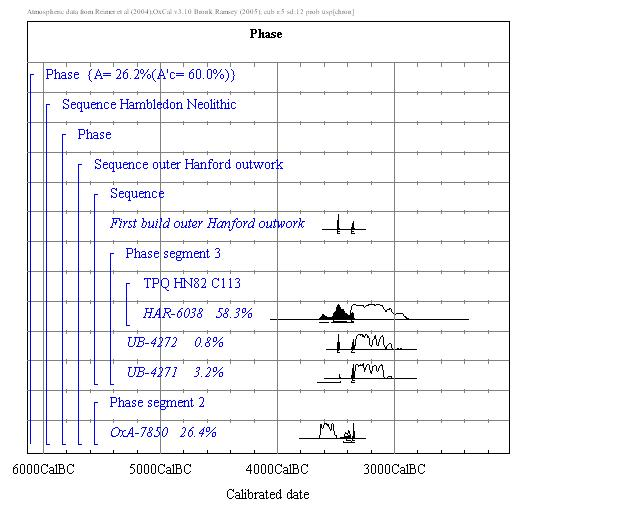
\includegraphics[width=0.9\textwidth]{figures/hanford-remodelled}
  \caption{Example OxCal output, from Hambledon Hill}
  \label{fig:hambledon-oxcal}
\end{figure}

This type of diagram is often used for the visual examination of the dates (see figure~\ref{fig:hambledon-oxcal} for an example) and is clearly completely aspatial. More generally, time is often referenced by specific period labels, as a series of successive snapshots, whose spatial features are then described, e.g. \citet[404]{Mercer:2008fk}. This is a very bland form of representation, simply listing phases by date does nothing to unravel the potential complexities of the temporality of the site. The snapshot representation could be enhanced, for example, by complementing with a more narrative approach, so emphasising the continual nature of change and the development of the site.

The snapshot model is entwined with the phasing of the site, it is well represented by a diagram taken from the report, reproduced in figure~\ref{fig:hambledon-earthworks}. This diagram demonstrates how the earthworks were built up during several phases of use, with each phase being presented as distinctly clear cut, with no representation of duration, or how long it took the changes enacted in each phase to be completed. There is also no clear connection between this plan and the bayesian model, the source of the date values.

\begin{figure}
\centering
	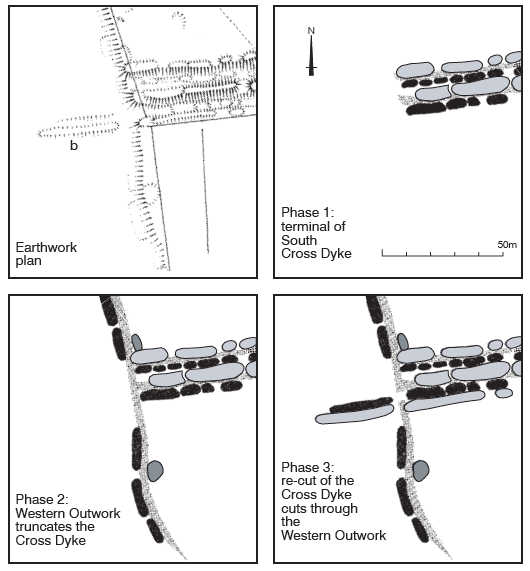
\includegraphics[width=0.9\textwidth,height=0.9\textheight,keepaspectratio=true]{figures/hambledon-earthworks2}
  \caption{Phasing of South Cross Syke, from \citet{Mercer:2008fk}}
  \label{fig:hambledon-earthworks}
\end{figure}

In many ways figure~\ref{fig:hambledon-devel} is similar, however it also demonstrates duration, by specifically identifying already existing features from the previous diagrams in the series, as well as the new ones for a particular phase. This is very similar to an example by Lucas, who suggests that as well as duration such a diagram allows the possibility of multiple phases existing at the same time, which in turn can be used to try and understand the experience of change \citep[41]{Lucas:2005fk}.

\begin{figure}
\centering
	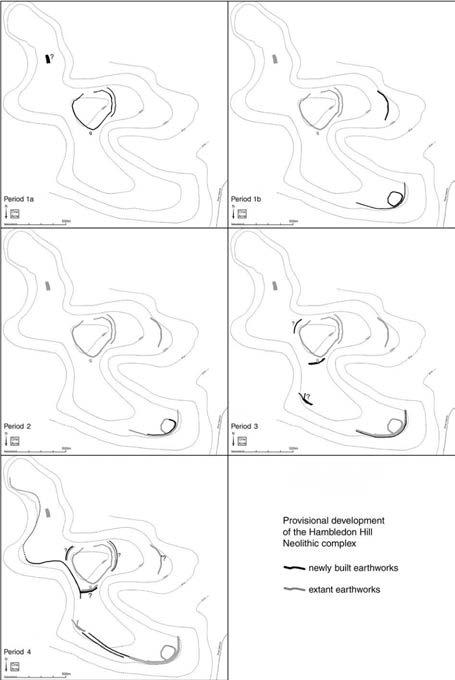
\includegraphics[width=0.9\textwidth,height=0.9\textheight,keepaspectratio=true]{figures/hambledon-devel}
  \caption{Development of Hambledon Hill from \citet{Mercer:2008fk}}
  \label{fig:hambledon-devel}
\end{figure}

These diagrams represent both space and time, which is a bit of a novelty in the Hambledon report and in archaeology more generally. In the reports chapter four, Interpreting Chronology, which covers the bayesian modelling of the radiocarbon dates and where most of the temporal analysis is documented, there are no plan diagrams. It is to all intents and purposes an a-spatial chapter. This is in contrast to chapter three, the excavation, which is in many respects a-temporal, where little chronology is provided, only a few section diagrams. From a narrative perspective, it would surely be inconceivable to divide space and time like this, both are a part of the same whole and complimentary to the story of the site. By separating space and time, it becomes more difficult to consider the continual nature (in time and space) of the processes of change, instead regarding change as the punctuation between specified snapshots.

While the benefits of applying bayesian modelling to individual sites, such as Hambledon, is obvious, they are clearly of limited value to wider questions. A series of studies have applied this method to multiple sites, providing the same benefits to the individual sites, but have also sought to address broader topics using this greater resolution of dating evidence. The original `Histories of the Dead' long barrow project \citep{CAJ:676016,CAJ:676116,CAJ:676124,CAJ:676132,CAJ:676140,CAJ:676148} uses bayesian modelling of radiocarbon dates to create finer chronologies for a group of long barrows, the results of which are then used to re-interpret the early Neolithic of southern Britain. The project was a precursor to `Gathering Time', \citep{Whittle:2011kl,Whittle:2011tg} a much larger project, focussing on 40 Neolithic enclosures in southern Britain, including Hambledon Hill, culminating in a re-appraisal of the temporal evidence for the early Neolithic in Britain. More recently `The Times of Their Lives' \citep{whittle2018times} applies these techniques to a large number of sites spread across continental Europe to address a range of theoretical issues. In these studies each site had its own specific research questions, the bayesian technique has helped answer these, in addition there were also overarching questions about the early Neolithic, such as ``When did causewayed enclosures begin to be built in Britain and Ireland'' \citep[13]{Whittle:2011kl}. 

For each of the individual site studies, there is often very limited spatial information. As an example, Hill Croft Field \cite[521]{Whittle:2011tg} contains no plan of the site at all. Between both Times of their Lives and Gathering Time, only one site has more than one plan, Fussells Lodge Long Barrow, in \citet{CAJ:676132} and they are rarely referred to. 

The data for both the radiocarbon determinations and the chronology at first glance appear distinctly absolute and un-problematic for input to a digital system. The radiocarbon being a probability distribution, and the chronology stored as a graph or tree type structure of nodes and relationships. Unfortunately, this line of reasoning leads straight into a trap; in many case studies, multiple models are given for each site because the models are based on an interpretation, there is no single version of the truth, only potential scenarios. If one were to simply take the preferred model and store it as `the' chronology for the site, this is taking something, which has an associated probability, and making it absolute and concrete. This is discussed in \citet{CAJ:676108} with reference to the quote on models often attributed to George Box - ``All models are wrong, some models are useful'' along with several techniques for determining the validity of different models. However, while it would be preferable to have certainty or quantified uncertainty, this is not always possible or ideal when dealing with multiple potential interpretations. Instead \citet{CAJ:676108} take a multiple pasts approach where the ``production of alternative models, none of them definitive, is simply a means of creating multiple pasts and is entirely congruent with the post-modern perspective'' \citep[5]{CAJ:676108}. The issues of exactness and the authority of computer generated results is clearly a crucial problem, as \citet[201]{Ramsey:2000fk} notes: \begin{quote}``there is no one correct prior for a given situation. A prior is merely a model that can be applied to the data to help in its interpretation. Ideally, several different models with different priors should be tried \ldots this approach may not appeal to some people who wish to take their results, process them statistically and come out with the `right'�� answer''.\end{quote} A pertinent quote to match that by George Box is one commonly attributed to John Tukey ``An approximate answer to the right problem is worth a good deal more than an exact answer to an approximate problem''.

Each of the individual studies has its own objectives, these objectives dictate the specific methods of analysis performed using the temporal data. The objectives are typically concerned with dating phases of construction and the duration of use, e.g. \citet[80]{Whittle:2011kl}. In addition, the results are combined to answer some more general questions about the British Neolithic, \citep[13]{Whittle:2011kl}, or to suggest connections between areas considered in the study, \citep[432]{Whittle:2011kl} and to challenge some specific theories or ideas, such as the connection between the continental LBK longhouses and British long barrows \citep[139]{CAJ:676156}. To answer these questions the primary form of analysis that has taken place is the bayesian technique, which combines the models and radiocarbon dates to create refined dates. This is also used to create the multiple pasts referred to above, based on the variations in the chronological model. Using the refined dates, further analysis is performed to examine durations, such as the number of years different part of a site were used for e.g. \citet[91]{Whittle:2011kl}. 

The topic of bayesian modelling of dates is not without controversy. In a recent review of the literature \citet{doi:10.1080/00438243.2015.1070082} split the main issues into ``whether the assumptions that underlie bayesian models are justifiable; and whether ��prior�� information essential to their construction (in this case, samples that have been dated) is relevant and reliable.'' \citep[527]{doi:10.1080/00438243.2015.1070082}. A large part of the study of each site is spent in justifying the inclusion or exclusion of samples (as recommended by \citealp{doi:10.1080/00438243.2015.1067640}) with any area of contention leading to the creation of multiple models, discussed in additional detail. The assumptions that underpin the model are generally presented textually, although in some studies stratigraphic relationships between samples are shown graphically, e.g. \citet[92]{CAJ:676140}. While such models as e.g. \citet[49]{CAJ:676124} are more stylised, in some publications the chronology presented to justify the bayesian model is similar to Harris-Matrix diagrams (e.g. \citealp[167]{AQY:9543450}). Clearly the validity of the model underpins any subsequent analysis performed on the results, it is therefore imperative to make sure such models are built on solid foundations. The problem is how to do this, \citet{doi:10.1080/00438243.2015.1070082} suggest that all models must be open to scrutiny \citep[14]{doi:10.1080/00438243.2015.1070082} which is clearly important for independent validation of results, and they also note it is important to select samples pertinent to the archaeological question \cite[4]{doi:10.1080/00438243.2015.1070082}. In this, Gathering Time is successful, their models and reasoning are published, although I am not aware of any independent validation of the results.

The next step is to consider how these projects represent time, including the results of the analysis. A large part of each study is devoted to a textual description of each of the samples and of the chronological model, with diagrams of the OxCal models, similar to those from Hambledon. Additional analysis such as durations are presented in a similar diagram generated by OxCal, the results from these diagrams are then used directly to answer the objectives of the studies. The multiple, alternative models are presented independently, with the preferred model being described in most detail, and other models gone through in a similar fashion, with particular focus on the areas that are different. This is a perfectly reasonable approach, although a graphical side-by-side representation would highlight the differences, and perhaps re-enforce the multiple realities aspect of multiple chronological models.

In the textual description of the temporal data, the authors convert their dates to life spans and generations, with life spans being set at 70 years, and generations set at 25 years \citep[16]{Whittle:2011kl}. These measures of time are then used to translate the output of the bayesian modelling into a format of date that has a more immediate human resonance, e.g. \cite[132]{CAJ:676156}. While this humanising of otherwise dry data is a welcome attempt at going from abstract chronologies to a more personal time scale, it is highly interpretative, not only the underlying dates, which are probabilities, and could easily not fit the neat small time spans of generations or life spans, but also the figures chosen to represent life spans and generations. Clearly, this is a what-if, an invite to picture how the monuments might resonate to a human time scale. In many ways, this type of interpretation is as much a form of representation of the temporal data as the graphical diagrams and models. It has been used successfully in other studies, 
\cite[e.g.][654]{doi:10.1080/00438243.2015.1053976} to contrast the prevailing view of conservatism with the dynamism implied by the results.

This representation is almost entirely a-spatial, a uni-dimensional representation of otherwise rich data, the reader could refer back to the (often) single plan, but this is not really enough, such a dimensionality reduction makes it much more difficult to analyse the changes or processes being included in the model. By leaving out the spatial data almost entirely it is difficult for the reader to become engaged in the analysis, the authors clearly known the proximity of the dates, but to anyone else they could all be at the exact same spot. Leaving out the spatial data makes it also nearly impossible to judge the scale of the site or sites being discussed. This is not uncommon in the bayesian literature,  \citet{doi:10.1080/00438243.2015.1053976} for example, only contains a map of Great Britain highlighting sites mentioned in the text, despite discussing in detail different parts of a key site. Combining time and space into a single diagram is difficult, but not a new problem \citet{Johnson:1999cr} mentions four methods often used by cartographers to include a representation of time in their diagrams, (see figure~\ref{fig:time-maps}) these being time slices, symbolism, arrows and difference maps. He refers to these methods as ``squeezing extra dimensions'' \citep[27]{Johnson:1999cr} out of two dimensional representations, and argues that they do not do justice to the underlying data, instead he recommends animation as it is a form or representation which makes use of time itself \citep[28]{Johnson:1999cr}.

\begin{figure}
\centering
	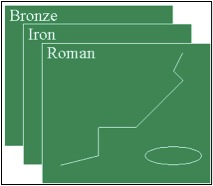
\includegraphics[width=0.4\textwidth]{figures/time-slices}
	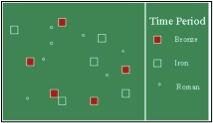
\includegraphics[width=0.4\textwidth]{figures/time-symbol}
	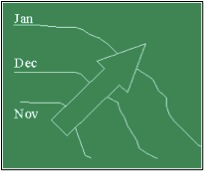
\includegraphics[width=0.4\textwidth]{figures/time-arrows}
	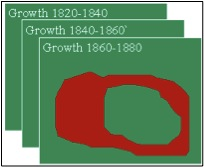
\includegraphics[width=0.4\textwidth]{figures/time-diff}
  \caption{Traditional methods of cartographic representation: a. Time slices; b. Symbolism; c. Arrows; d. Difference maps, from \citet{Johnson:1999cr}}
  \label{fig:time-maps}
\end{figure}

More recently \citet[7]{lock2002analysing} suggested a 3D method which would also permit the uncertainty of dates to be displayed as part of the diagram, by including a 3rd axis (in additional to two spatial) where the less likely a site is of being in use, the less clearly it is drawn (for example dashed or dotted lines for features are used instead of uninterrupted ones). Both of these proposals have serious issues, which will be examined in more detail later on in this study, for now let us briefly consider them. Animation as a form of representation might be suited to showing objects or events with certain dates, but once these dates become probabilistic, it will soon become an unclear mess of many objects or events. These events may or may not even have occurred simultaneously, potentially creating a false sense of synchronicity between events, which in fact did not occur at the same time. A similar problem exists with representing the probability of use as a third axis, in this case it will be easier to see that events may not be concurrent. But with more than a few dates, especially with overlapping spatial data, the diagram will rapidly become unreadable. That none of these techniques has been used in practice to include a representation of time with spatial data is a shame, as experimentation can lead to innovation, but it also suggests that the problem is perhaps a tricky one, and that a bit of cartographic magic will not do full justice to the underling data.

In some respects there are parallels with what \citet{Rennell2012} has termed subject-centred landscape archaeology. In such studies, diagrams often take a back seat role, compared to the detailed textual description. An example of this is \citet{Vavouranakis:2006fk} which features a descriptive study of the landscapes of the town of Gournia, a ``series of meaningfully constructed landscapes, ranging from the personal, familiar, and mundane to the economic, political, ritual, and exceptional'' \citep[237]{Vavouranakis:2006fk} and of how these landscapes developed over time. It focused on how societal changes may be being reflected in changes to buildings, presented in a broad narrative, with only a couple of maps to provide context. By considering change over time, that study was moving towards a more integrated spatio-temporal analysis, but unlike the more exclusively temporal studies mentioned above, it focuses on spatial elements by taking a (spatial) narrative approach to moving through the landscape. Crucially the narratives are presented sequentially, as a textual snapshot based model, one for early, middle and late Bronze Age. There is little consideration for the process of change, only a description of those changes. Clearly this approach would benefit from the addition of a temporal narrative, a description of the interplay between the eras, and of how past, present and future should be just as much the targets of a subject-centred study. While this kind of approach has a lot to offer, I'm not convinced that it would make full use of the refined dates and multiple pasts created by bayesian techniques. Fortunately, \citet{Rennell2012} also demonstrates several techniques for combining methods of subject-centred survey with more traditional spatial analysis, such as comparing visibility on the ground with computed viewsheds, and augmenting continuous viewsheds with details of journeys through the landscape. By combining techniques in this way a more holistic interpretation and analysis is possible, something lacking with current temporal techniques.

The field of spatial analysis has several parallels with the kind of temporal analysis reviewed above, there are different types of data, vector and raster, a range of statistical analysis techniques, and a need for specialist software. A key difference between the two areas is the available methods, where as the spatial analyst has a toolbox of techniques including spatial searches, digital elevation models, clustering, autocorrelation, viewsheds, etc, there is a paucity when it comes to temporal equivalents. Bayesian modelling is clearly a powerful technique, which can be used not only to refine dates, but also to examine chronologies, calculate durations of use, or inactivity. In addition, there are other temporal methods, such as summing radiocarbon dates, or the chi-squared approach to wiggle matching, however, some of these appear to have been in decline in recent years \citep[678]{doi:10.1080/00438243.2015.1067640}. Ultimately these methods are about refining the data, unlike the spatial techniques, which are about highlighting information that is not immediately apparent in the data. The field of temporal analysis is arguably only just beginning to flourish, especially bayesian modelling of dates, where the majority of papers have only been published in the last five years (as of 2015) \citep[678]{doi:10.1080/00438243.2015.1067640}.

Clearly, the archaeological questions asked dictate the analytical methods used, up to now the kinds of questions asked of temporal data are familiar. For example \citet{CAJ:676116} looks to: determine if there is a gap between Mesolithic and Neolithic occupation, and if so for how long; to determine a date and duration for the Neolithic occupation; to see if there was a gap between occupation and barrow construction; to date the contraction of the monument; to determine the duration of infilling of ditches; to date the barrow extension; and to date the burial activity in the cists. These kinds of questions fall into two categories, questions of date and questions of durations. For these kinds of questions, the bayesian methods are clearly appropriate, providing more detailed answers than previous methods. However, these are the same kinds of questions that have been asked of temporal data for a long time. For the field of temporal analysis to expand and flourish, it is crucial to start asking other kinds of questions, which will lead to new forms of analysis. And it will be essential to engage with theoretical questions, a prime (non-temporal) example of this is \citet{Evans:2006fk}, which analysed the identity prescribed to individuals based on grave goods in Iron Age France, specifically notions of gender and social standing. Using the mean frequency of artefacts Evans was able to show that burials with engendering grave goods assemblages were likely to have more goods overall, implying a higher social prestige \citep{Evans:2006fk}. In addition, the statistical analysis was able to demonstrate a change in goods frequencies over time, implying a change in the nature of status and in gender roles. Evans took the statistical results, and linked them to theoretical issues of status, going from descriptive to the interpretative. This is important for temporal analysis, it is already happening, slowly, for example in \citet{CAJ:676156} the issue of the influence of continental long houses on British long barrows is discussed. But more could be done in this area to make this kind of question the ultimate objective, and make the determination of dates just a step down the path.

To recap, there is a burgeoning field of temporal analysis, several example studies with a temporal focus have been examined in detail, and many other studies drawn on. They shared common forms of temporal data, primarily radiocarbon dates and chronology, and common methods of temporal analysis. This analysis is mostly based upon bayesian modelling of dates, which has been used to answer typical questions of age and duration. This technique is not without its problems. While mathematically rigorous it requires interpretation for the construction of chronologies and its graphical outputs are not always straightforward to interpret. It also leads to the creation of multiple models, which may be problematic. Temporal data has generally been presented in a textual, a-spatial format, often accompanied by technical diagrams from bayesian modelling software. This is a clear limitation of current approaches, with the lack of any spatial element going right through the process, all the way back to data collection, where it is treated independently from temporal data. Perhaps this is considering spatiality and temporality as being two sides of the same coin, however we should also surely be considering the coin as a whole. The next step for archaeological temporal analysis is to include the spatial information, so that it becomes spatio-temporal analysis, to unify both sides of the coin. Only by combining the two will it be possible to fully utilise the temporal data available. 

Such analysis is a rare thing in Archaeology, but not wholly unheard of, for example a series of studies have looked at the spatio-temporal patterns of the Lowland Classic Maya collapse \citep{Bove:1981fk,Whitley:1985uq,Kvamme:1990kx}. In the initial study, \citet{Bove:1981fk} constructed several trend surfaces (see figure~\ref{fig:bove-map} for an example) for the dates of the latest stelae (stone monuments) at each settlement. Trend surfaces are usually a tool for spatial analysis, and are a means of fitting a function through a set of values \citep{Bove:1981fk}. In this case, the values are the date of erection of the last stone monuments, with the height of the surface calculated based on these dates, so the spatial trend was a temporal one, showing where the end of construction of these monuments started, and how it spread spatially. Using this technique, Bove was able to argue for a regional approach to the collapse \citep[111]{Bove:1981fk}, with outside groups possibly moving in to exploit a power vacuum \citep[110]{Bove:1981fk}. This analysis was then verified using spatial autocorrelation, firstly by \citet{Whitley:1985uq} who attempted to demonstrate that no simple geographic pattern existed, \citep[390]{Whitley:1985uq} and then later by \citet{Kvamme:1990kx} who showed that such a pattern did exist \citep[203]{Kvamme:1990kx} and that the technique employed in \citet{Whitley:1985uq} was unsuitable for the data \citep[201]{Kvamme:1990kx}. 

\begin{figure}
\centering
	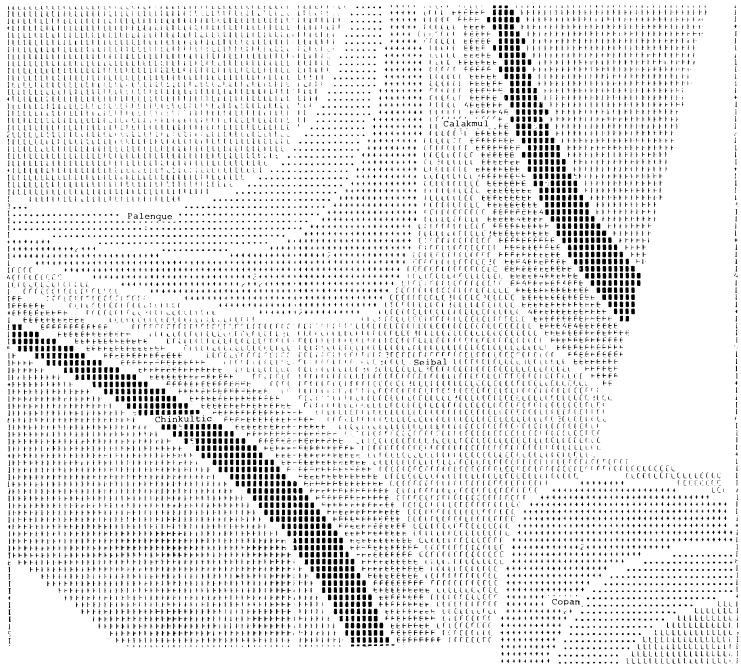
\includegraphics[width=0.9\textwidth]{figures/maya-1}
  \caption{Second-order trend surface contour map, from \citet{Bove:1981fk}}
  \label{fig:bove-map}
\end{figure}

Such interesting analysis would not be possible if space and time had been considered independently, by combining them in this way it has been possible to learn much more about the Lowland Classic Maya collapse. In order to combine both space and time in this case, spatial techniques have been applied using temporal data as an attribute, for the trend surface, a z-axis value. This is a straightforward approach using existing, already tried and tested methods with appropriate spatio-temporal data. The difficulty in performing spatio-temporal analysis like this more broadly is in having temporal data that can be used. Fortunately, there is high-resolution temporal data for the erection dates of the Maya stone monuments that enables these dates to be presented as specific years on our calendar. A lot of archaeological temporal data does not fit into this exact, historical form, being less certain, in many cases probabilistic. In order to easily perform analysis, which is repeatable, and combines both spatial and temporal data we will require the use of specialist methods that can cope with archaeological temporal data and software to perform analytical techniques.

Fortunately within archaeological Geographic Information System (GIS) studies, there is a seam of research into Temporal GIS (TGIS). This would provide software that could operate on spatial data as a GIS does, but could also incorporate temporal data, and perform operations and analysis on combined spatio-temporal data that go beyond treating time as an attribute of spatial data, elevating it to being an equal part of the analytical technique. Such a system would also be capable of comprehending and working with the types of temporal data archaeologists have available. 

This brief overview has toured both method and theory of spatio-temporal analysis at both a small and large scale. It has shown that to gain maximum benefit from spatio-temporal research, the necessity to re-contextualise the temporal data with its corresponding spatial component. The subject has been approached from a temporal perspective, taking the site of Hambledon Hill to understand the full life cycle of temporal data, ultimately, from it's place in the ground, to the regional analysis of Gathering Time. The theories and methods of spatio-temporal analysis are relevant throughout that life cycle. This introduction to the topic has identified three key components in the study of spatio-temporal data, in fact all archaeological data. By examining each of these components in turn, we will not only understand the state of the art of the subject, but will be in a position to enhance the value that can be obtained from the analysis of archaeological data. 
\begin{enumerate}
\item Asking the right questions -
as mentioned above, the questions dictate the methods, therefore it is important to at least start to address them first. In order for the field of temporal analysis to progress, it is crucial to move from descriptive questions to those of a more analytical or interpretative nature. This component will consider what kinds of questions are asked of temporal data, with an aim of enhancing such questioning by an inclusion of the spatial dimension.
\item Analytical techniques -
next, it is necessary to consider what methods are available to analyse the data, the validity and the general acceptance of those methods. We must also consider whether the currently available methods will actually help answer our questions, or if new methods will be required. Finally, it is important to consider the correct application of such methods, as without this how can the validity of any results be ensured?
\item Spatio-temporal software -
specialist software will be required to handle the data and perform the analysis, as current GIS platforms do not handle the probabilistic dates of archaeology. This chapter will review the available options, and determine if any can be used out of the box, or if not, what can be learnt about the most effective way of meeting these technical requirements.
\end{enumerate}